\documentclass[journal]{IEEEtran}
\usepackage[T1]{fontenc}
\usepackage{amsmath,amsfonts,amssymb}
\usepackage{algorithmic}
\usepackage{algorithm}
\usepackage{array}
\usepackage[caption=false,font=normalsize,labelfont=sf,textfont=sf]{subfig}
\usepackage{textcomp}
\usepackage{stfloats}
\usepackage{url}
\usepackage{verbatim}
\usepackage{graphicx}
\usepackage{cite}
\usepackage{bm}
\usepackage{multirow}
\usepackage{balance}

\newtheorem{proposition}{Proposition}
\newtheorem{theorem}{Theorem}

\hyphenation{op-tical net-works semi-conduc-tor IEEE-Xplore}

\begin{document}

\title{Pragmatics-Aware Token Selection and Scheduling for Generative Semantic Communication over Time-Varying Channels}

\author{Changyu~Zhang, Lingyun~Lu, Wei~Ni,~\IEEEmembership{Senior Member,~IEEE}, Xiaoqiang~Zhu,~\IEEEmembership{Member,~IEEE}
\thanks{Changyu~Zhang and Lingyun~Lu are with the School of Software Engineering, Beijing Jiaotong University, Beijing 100044, China (e-mail: 25121368@bjtu.edu.cn; lylu@bjtu.edu.cn). (Corresponding author: Changyu~Zhang.)}
\thanks{Wei~Ni is with the School of Engineering, Edith Cowan University, Perth, WA 6027, Australia (e-mail: wei.ni@ieee.org).}
\thanks{Xiaoqiang~Zhu is with the School of Cyberspace Science and Technology, Beijing Jiaotong University, Beijing 100044, China (e-mail: xqzhu@bjtu.edu.cn).}}

\markboth{IEEE Transactions on Vehicular Technology}%
{Zhang and Lu: Pragmatics-Aware Token Selection and Scheduling for GSC over Time-Varying Channels}

\maketitle

\begin{abstract}
Generative semantic communication (GSC) achieves efficient transmission by converting multi-modal content into prompts. Yet, existing methods treat a prompt as a monolithic unit and do not differentiate individual token importance under time-varying channels. We propose a token-level pragmatics-aware selection and adaptive scheduling method. A unified pragmatic metric combines causal self-attention, semantic directional consistency, and deletion-aware gradient sensitivity. A direction-preserving coupling model then evaluates the utility of the actually received token set, rather than summing token scores precomputed on the full prompt. Under imperfect channel state information (CSI), token selection and coding protection are jointly optimized using conditional decoding probabilities and reliable channel capacity. Lagrangian relaxation solves the additive linear relaxation, certified extreme-point rounding constructs a feasible schedule, and coupling-aware local refinement improves it. In multi-terminal scenarios, online semantic prices and reliable spectral efficiencies determine the bandwidth allocation through a proportional-fair objective. The analysis establishes a token-scale semantic proxy bound, an explicit rate--retention--VQA boundary, a model-mismatch bound, an approximation guarantee, and an end-to-end performance decomposition that jointly accounts for optimization, semantic approximation, model variation, and channel outage.
\end{abstract}

\begin{IEEEkeywords}
Dynamic prompt pruning, generative semantic communication, semantic coupling, time-varying channel scheduling, token-level pragmatic metric.
\end{IEEEkeywords}

\section{Introduction}
\IEEEPARstart{T}{he} explosive growth of image and video traffic from intelligent terminals has pushed conventional bit-accurate communication toward its information-theoretic ceiling. Semantic communication (SC)~\cite{gunduz2023beyond} represents a paradigm shift that transmits task-relevant semantics rather than raw bits, treating the encoder and decoder as cooperative inference modules rather than waveform reproducers. Early SC realizations adopt deep joint source-channel coding (DeepJSCC) to map signals into feature vectors~\cite{bourtsoulatze2019deep}, with notable progress in single-modal tasks and task-oriented multi-user scenarios~\cite{xie2021task}. The feature dimensionality required for high-dimensional multi-modal content remains substantial. Generative semantic communication (GSC) reduces this cost by one to two orders of magnitude~\cite{Qiao2024latency,ren2025generative}: the transmitter uses a vision-language model (VLM) to convert multi-modal inputs into compact natural-language prompts, and the receiver reconstructs semantic content via a diffusion model or a large language model (LLM). Within a prompt, however, tokens contribute unevenly to the output, and their relative importance further varies with the instantaneous channel state.

Existing studies have approached this problem from complementary perspectives. Information-bottleneck criteria~\cite{shao2021learning} offer principled tools for semantic feature selection, while fading-robust DeepJSCC~\cite{Yang2022ofdm} and online-adaptive transform-based transmission~\cite{daiTowardAdaptive} improve resilience under channel fluctuations. Multi-terminal SC~\cite{yang2025rethinking}, joint user association with bandwidth allocation~\cite{xia2023joint}, and large AI model-empowered multimodal SC~\cite{jiang2025large} broaden the applicability of SC systems. Despite this progress, four gaps remain. First, semantic importance is typically modeled at the feature or prompt level, leaving intra-prompt token heterogeneity unexploited. Second, a token score evaluated on the full prompt is often added after pruning, although its contextual support may have been removed. Third, imperfect CSI, differentiated coding, and residual decoding errors are rarely represented in the same token utility. Fourth, multi-terminal bandwidth allocation rarely reflects the marginal semantic value of bandwidth, so that terminals with urgent content can be starved while those with redundant content waste channel resources.

\begin{figure*}[t]
\centering
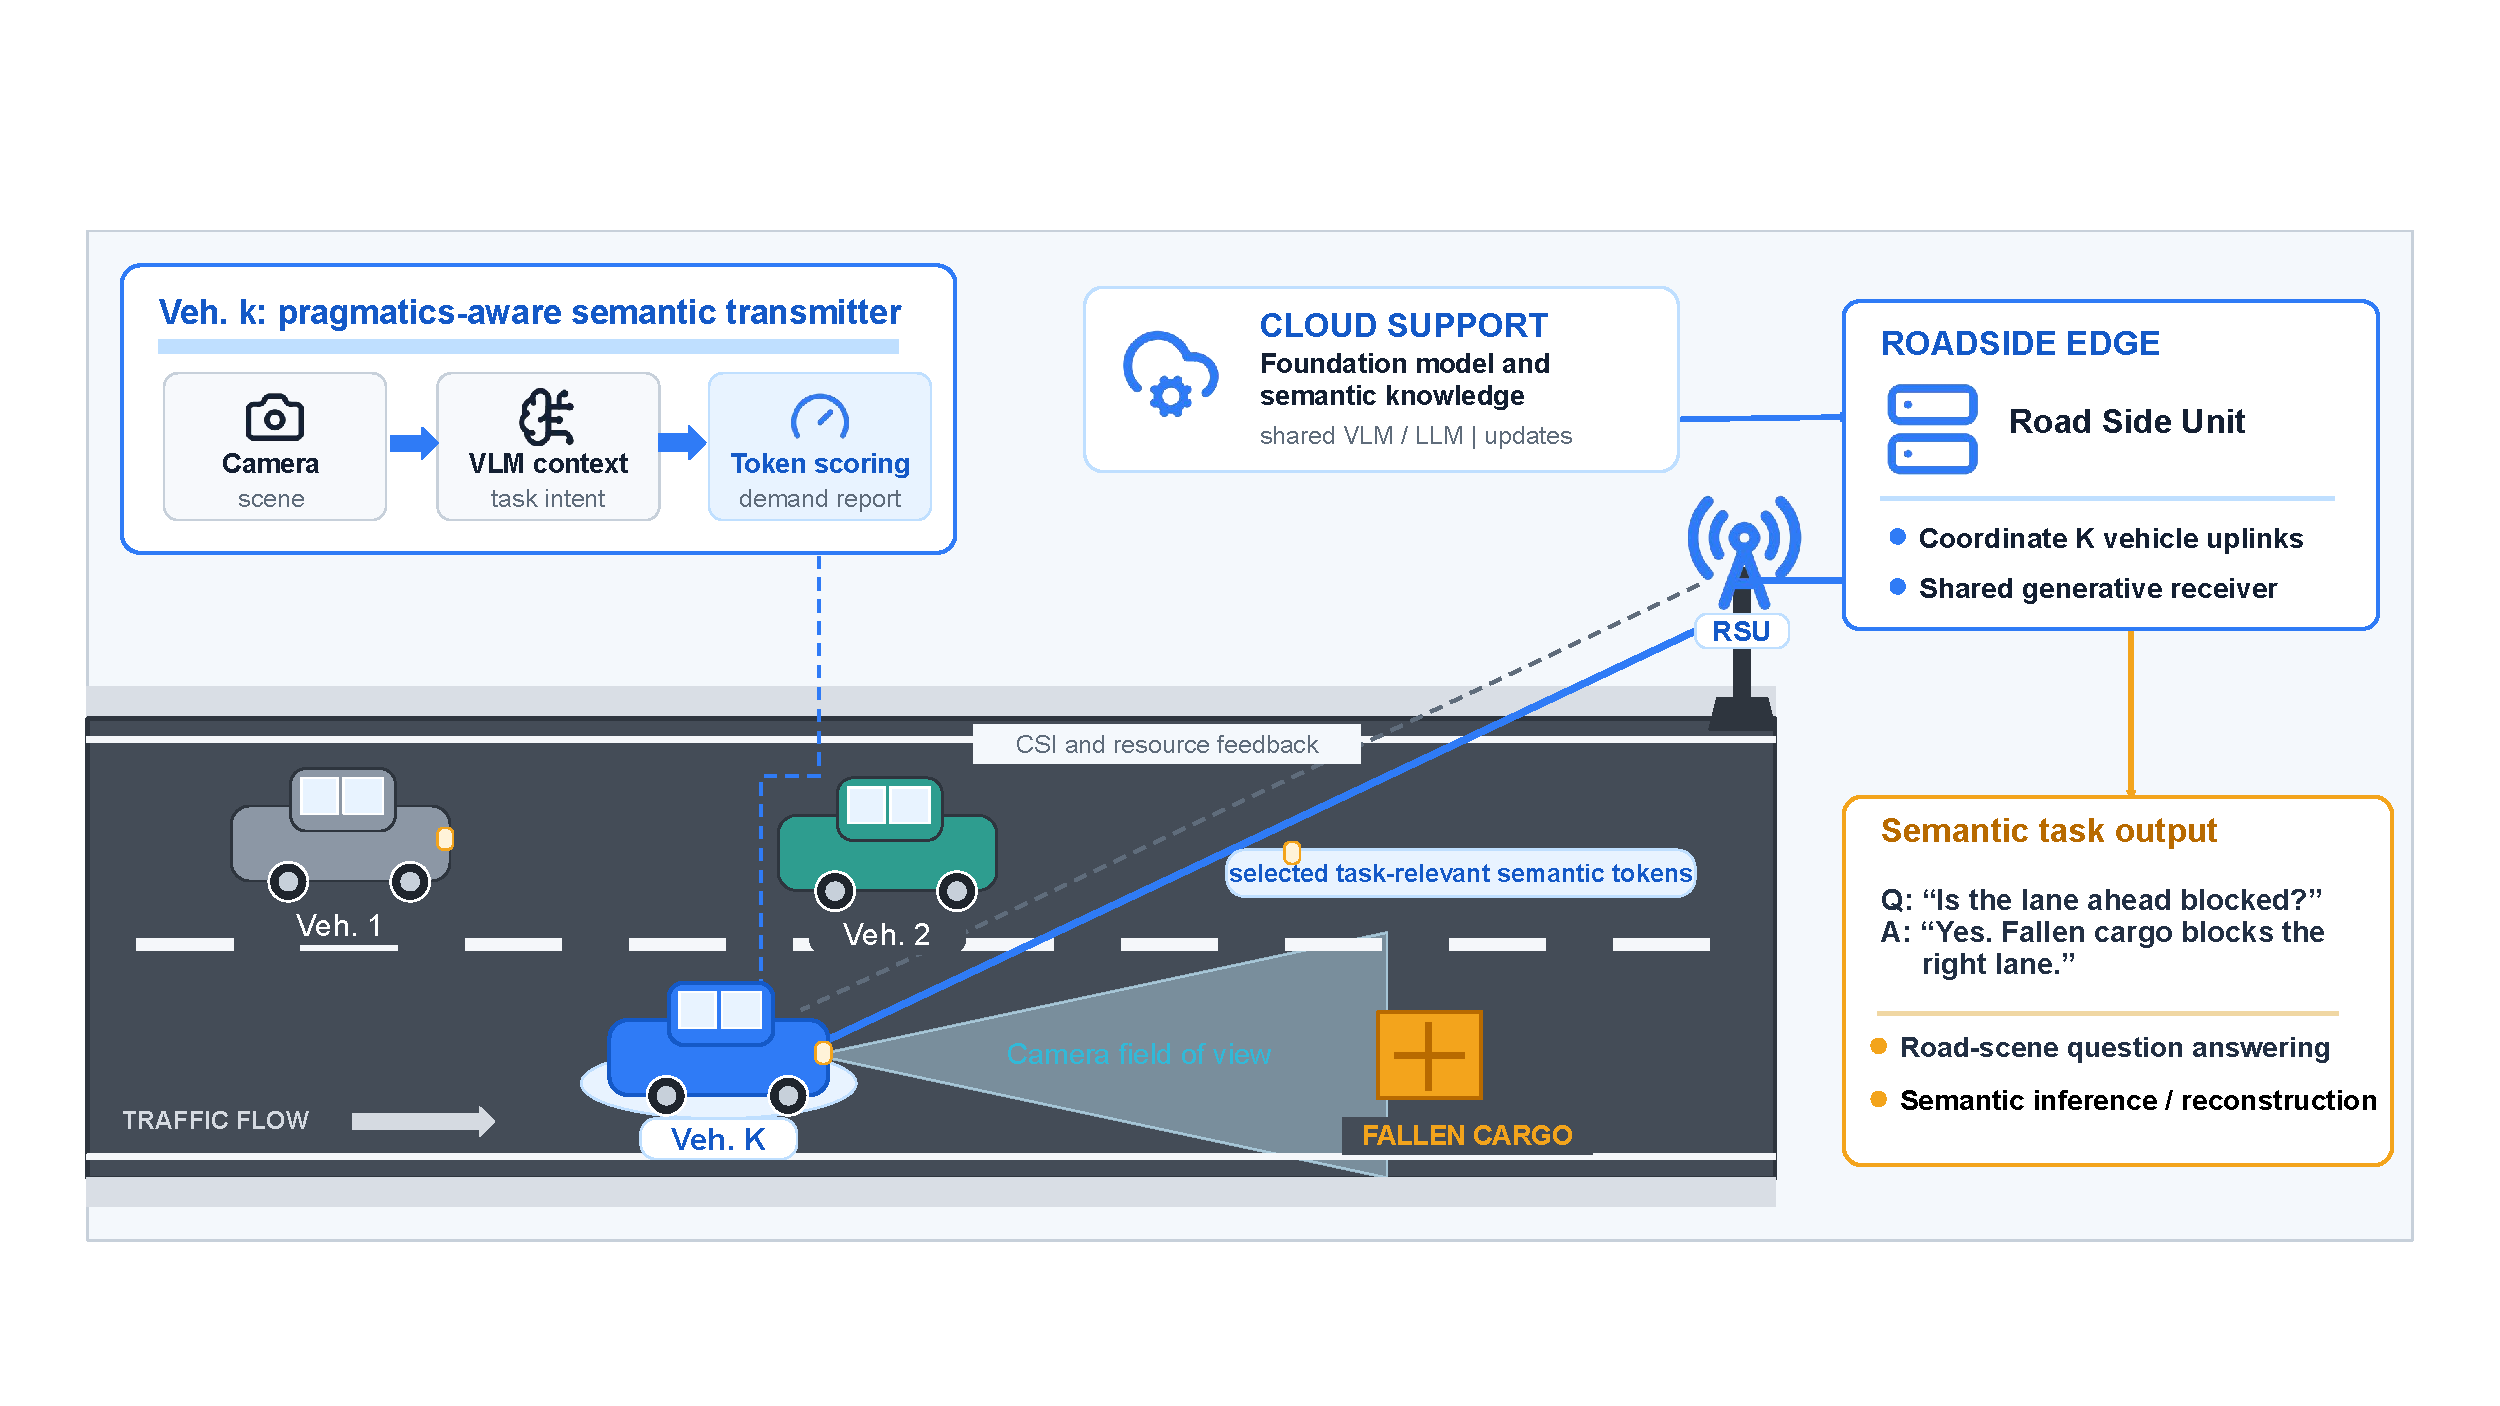
\includegraphics[width=0.96\textwidth,trim=0 32 0 40,clip]{images/vehicular_application_scenario.pdf}
\caption{Representative vehicular deployment of the considered shared-uplink GSC system. Each vehicle first performs local semantic extraction and pragmatic scoring, and reports a compact semantic demand to the roadside unit. The roadside unit coordinates the $K$ vehicle uplinks and returns resource grants; each vehicle then finalizes token selection and protection before transmitting the semantic payload. Cloud support supplies foundation-model and semantic-knowledge updates outside the per-slot scheduler.}
\label{fig:vehicular_scenario}
\end{figure*}

A representative deployment is illustrated in Fig.~\ref{fig:vehicular_scenario}. Each connected vehicle locally converts its camera observation and task intent into a prompt and evaluates token utility before requesting radio resources. This preparation does not transmit the candidate tokens. The roadside unit obtains the uplink CSI, combines it with a compact terminal-level semantic demand, and returns a resource grant. The vehicle then finalizes token selection and protection under that grant, and only the selected task-relevant tokens enter the data uplink. The cloud may distribute model and semantic-knowledge updates at a slower time scale, but it is not required by the online token and bandwidth decisions developed below.

To bridge these gaps, this paper presents a pragmatics-aware token-level selection and adaptive scheduling method for time-varying multi-terminal GSC. The main contributions are as follows:
\begin{itemize}
\item We design a multi-dimensional pragmatic contribution metric that fuses self-attention structural weights, semantic directional consistency, and deletion-aware generative gradient sensitivity. A Taylor bound relates the gradient term to the task-loss increment caused by token removal.
\item We design a direction-preserving semantic coupling model whose utility depends on the actually received token set. The resulting marginal gains remove the unselected-token leakage of a full-prompt pre-score, and a second-order bound characterizes the semantic proxy error.
\item We jointly select tokens and coding protection under imperfect CSI. Conditional decoding probabilities and a reliable channel budget enter the same expected semantic objective. Lagrangian breakpoint search and certified LP extreme-point rounding provide a feasible initializer with a proved factor, which coupling-aware local refinement can only improve.
\item We design a multi-terminal scheduling scheme in which online semantic prices track time-varying resource pressure. A proportional-fair objective yields a bandwidth allocation governed by marginal semantic benefit and reliable spectral efficiency. A rate--retention--VQA boundary and approximation, model-mismatch, channel-outage, price-error, and complexity bounds are also established.
\end{itemize}

The rest of this paper is organized as follows. Section~\ref{sec:system} presents the task and channel models. Section~\ref{sec:utility} develops the token and set-level semantic utility. Section~\ref{sec:optimization} formulates and solves the reliability-aware joint scheduling problem. Section~\ref{sec:analysis} provides performance and complexity analyses. Section~\ref{sec:exp} specifies the experimental evaluation, and Section~\ref{sec:conclusion} concludes the paper.

\section{System Model and Problem Formulation}
\label{sec:system}

\subsection{Multi-Terminal Prompt Transmission and Task Loss}

\begin{figure*}[t]
\centering
\includegraphics[width=\textwidth]{images/gsc_architecture.pdf}
\caption{Multi-terminal pragmatics-aware GSC architecture and token contribution evaluation. Each terminal performs VLM encoding and local pragmatic evaluation, and sends a compact semantic-demand report $p_k$ to the joint bandwidth allocator. The coordinator combines the reports with CSI and returns a reliable resource budget, after which each terminal prunes and protects its tokens for uplink transmission. The lower panel illustrates the fusion of structural dependency, semantic representation, and task-loss sensitivity followed by semantic coupling correction. In the formulation below, $p_k$ is instantiated by the marginal semantic report derived from $\mu_{k,\tau}$, and the allocated resource is represented by $C_{\tau}^{(k)}$.}
\label{fig:framework}
\end{figure*}

The processing chain is detailed in Fig.~\ref{fig:framework}. We consider $K$ uplink terminals sharing one receiver; the vehicles and roadside receiver in Fig.~\ref{fig:vehicular_scenario} provide one representative realization. Terminal $k$ converts an image $I_k$, a question $Q_k$, and related context into a prompt
\begin{equation}
\mathcal{P}^{(k)}=\{w_1^{(k)},\ldots,w_{N_k}^{(k)}\},
\qquad
\bm e_i^{(k)}\in\mathbb{R}^{d}.
\label{eq:prompt}
\end{equation}

The control and data flows are separated as follows. First, each terminal performs VLM inference, pragmatic scoring, and coupling evaluation locally, and forms a scalar semantic-demand report $p_{k,\tau}$ from its current semantic price; neither token embeddings nor a candidate token set are uploaded in this phase. Second, the terminal sends $p_{k,\tau}$ on a reserved low-rate uplink control resource, while the receiver obtains uplink CSI from pilots or sounding reference signals. These preconfigured control resources are not part of the semantic data budget optimized below. Third, the receiver jointly allocates the shared time--frequency resource across the $K$ terminals and returns $B_{k,\tau}$ together with the applicable link-mode information on the downlink control channel. Finally, terminal $k$ uses this grant to select token--protection pairs and transmits the resulting protected token payload on the scheduled uplink data channel. The receiver channel-decodes the payload and invokes the generative task model.

Thus, semantic importance and the final per-token protection decision remain at the terminal, where the token content is available. The receiver determines the inter-terminal resource budget and the feasible link-adaptation options. Their combination makes the overall optimization joint without requiring centralized inspection of every token. The successfully decoded tokens are used for answer generation or visual question answering. This setting corresponds to multiple terminals sharing one uplink receiver, rather than a general multi-pair network. Extending the formulation to a true multi-transmitter--multi-receiver network would require a receiver index, transmitter--receiver association variables, interference-coupled signal-to-interference-plus-noise ratios, and receiver-specific semantic mismatch terms. These additions destroy the per-terminal separability used by the present token selector and bandwidth KKT condition; joint association, interference management, and scheduling are therefore outside the scope of this work.

Let $\bm\theta_{\mathrm T}^{(k)}$ and $\bm\theta_{\mathrm R}$ denote the transmitter-side proxy model and the receiver-side task model, respectively. For a target answer sequence $\bm y_k^\star=\{y_{k,1}^\star,\ldots,y_{k,T_y}^\star\}$, the autoregressive negative log-likelihood (NLL) of model $m\in\{\mathrm T,\mathrm R\}$ is
\begin{equation}
\mathcal L_m^{(k)}(\mathcal P)
=-
\sum_{t=1}^{T_y}
\log p_{\bm\theta_m^{(k)}}
\!\left(
y_{k,t}^\star\mid \bm y_{k,<t}^\star,I_k,Q_k,\mathcal P
\right),
\label{eq:task_loss}
\end{equation}
where $\bm\theta_{\mathrm R}^{(k)}=\bm\theta_{\mathrm R}$ is used for notational consistency. The system ultimately seeks to reduce $\mathcal L_{\mathrm R}^{(k)}$, but the transmitter generally cannot access receiver-side gradients. Token scores are therefore constructed from $\mathcal L_{\mathrm T}^{(k)}$ and connected to receiver performance through a model-mismatch bound.

For multiple-choice VQA, an incorrect maximum-probability answer implies that the probability of the correct answer is no larger than $1/2$. Hence,
\begin{equation}
\mathbf 1\{\widehat y_k\neq y_k^\star\}
\leq \frac{\mathcal L_{\mathrm R}^{(k)}}{\log 2},
\qquad
\Pr(\widehat y_k\neq y_k^\star)
\leq \frac{\mathbb E[\mathcal L_{\mathrm R}^{(k)}]}{\log 2}.
\label{eq:vqa_error_bound}
\end{equation}
The theoretical objective is thus not to assume a linear relation between a gradient norm and VQA accuracy. It is to control the NLL increment caused by token removal and transmission failure, which in turn controls an interpretable upper bound on the VQA error probability.

\subsection{Time-Varying Channel and Reliable Capacity}

Let $h_{\tau}^{(k)}\in\mathbb C$ denote the channel coefficient of terminal $k$ in slot $\tau$. Imperfect CSI is modeled as
\begin{equation}
\widehat h_{\tau}^{(k)}=h_{\tau}^{(k)}+e_{\tau}^{(k)},
\qquad
e_{\tau}^{(k)}\sim\mathcal{CN}(0,\sigma_e^2).
\label{eq:csi}
\end{equation}
The channel may follow Rayleigh, Rician, frequency-selective, or ray-tracing distributions. The analysis only requires the conditional distribution of $h_{\tau}^{(k)}$ given $\widehat h_{\tau}^{(k)}$, or a conservative lower confidence bound derived from recent channel observations.

Capacity with channel side information depends on which terminals know the channel and on the quality of that information~\cite{goldsmith1997capacity,medard2000imperfect}. Directly inserting $\widehat h_{\tau}^{(k)}$ into the perfect-CSI Shannon expression treats the estimate as the true channel and is therefore optimistic under estimation error. For an allowed outage probability $\varepsilon_{\mathrm{out}}$, we instead define the conditional reliable spectral efficiency as
\begin{align}
c_{\varepsilon}^{(k)}(\widehat h_{\tau}^{(k)})
=\sup\big\{c:~&\Pr[\log_2(1+\bar\gamma|h_{\tau}^{(k)}|^2)\geq c
\mid \widehat h_{\tau}^{(k)}]
\notag\\[-0.2em]
&\geq 1-\varepsilon_{\mathrm{out}}\big\},
\label{eq:reliable_spectral_efficiency}
\end{align}
where $\bar\gamma$ is the average SNR. We use one equivalent-bit coordinate throughout the paper. If terminal $k$ receives bandwidth $B_{k,\tau}$ over a slot of duration $T_s$, its reliable budget is
\begin{equation}
C_{\tau}^{(k)}
=T_sB_{k,\tau}c_{\varepsilon}^{(k)}(\widehat h_{\tau}^{(k)}).
\label{eq:reliable_capacity}
\end{equation}
The numerical evaluation normalizes $T_s=1$ only after the units in~\eqref{eq:reliable_capacity} are fixed. To protect against channel-distribution shift, let $\mathfrak P_{k,\tau}$ be an ambiguity set of plausible conditional laws of $h_{\tau}^{(k)}$ given $\widehat h_{\tau}^{(k)}$, constructed from recent channel observations, and write $\psi_{k,\tau}(h)=\log_2(1+\bar\gamma|h|^2)$. A distributionally robust alternative is
\begin{equation}
\begin{split}
c_{\varepsilon,\mathrm{rob}}^{(k)}
\big(\widehat h_{\tau}^{(k)}\big)
\triangleq
\inf_{\mathbb Q\in\mathfrak P_{k,\tau}}
\sup\big\{c:\;&
\mathbb Q\big[
\psi_{k,\tau}(h_{\tau}^{(k)})\geq c
\mid\widehat h_{\tau}^{(k)}
\big]
\\[-0.2em]
&\geq1-\varepsilon_{\mathrm{out}}\big\}.
\end{split}
\label{eq:robust_reliable_spectral_efficiency}
\end{equation}
Replacing $c_{\varepsilon}^{(k)}$ in~\eqref{eq:reliable_capacity} with~\eqref{eq:robust_reliable_spectral_efficiency} gives the worst-case reliable budget over $\mathfrak P_{k,\tau}$. If the unknown test-channel law $\mathbb Q_{k,\tau}^{\star}$ belongs to $\mathfrak P_{k,\tau}$ with confidence at least $1-\delta_{\mathrm{amb}}$, then, with the same confidence,
\begin{equation}
\Pr_{\mathbb Q_{k,\tau}^{\star}}
\!\left[
T_sB_{k,\tau}\psi_{k,\tau}(h_{\tau}^{(k)})
<C_{\tau,\mathrm{rob}}^{(k)}
\mid\widehat h_{\tau}^{(k)}
\right]
\leq\varepsilon_{\mathrm{out}}.
\label{eq:distribution_shift_outage}
\end{equation}
A singleton ambiguity set recovers~\eqref{eq:reliable_spectral_efficiency}; an empirical lower-confidence quantile or a statistically calibrated ambiguity radius yields an online implementation without assuming that the test-channel distribution matches the distribution used for parameter selection.

Let $\mathcal R=\{H,M,L\}$ denote the available protection levels. The equivalent-bit cost of transmitting token $i$ from terminal $k$ at level $\ell$ is $r_{i\ell}^{(k)}$, with $r_{iH}^{(k)}>r_{iM}^{(k)}>r_{iL}^{(k)}>0$. The binary variable $y_{i\ell,\tau}^{(k)}=1$ selects this token--protection mode, and
\begin{equation}
\sum_{\ell\in\mathcal R}y_{i\ell,\tau}^{(k)}\leq 1.
\label{eq:one_mode}
\end{equation}
Given the current CSI, $q_{i\ell,\tau}^{(k)}$ denotes the conditional probability that this mode is successfully decoded. Packet loss, residual channel-decoding errors, and the protection level are all absorbed into $q_{i\ell,\tau}^{(k)}$.

\subsection{Unified Assumptions}

The task loss is assumed to be twice differentiable with respect to the concatenated token embeddings, with a bounded and locally Lipschitz Hessian. The structural and coupling coefficients used below are extracted from masked self-attention in an autoregressive decoder under teacher forcing; consequently, a query at position $j$ can attend only to keys at positions $i<j$. A model exposing only bidirectional encoder attention does not satisfy this causal-attention assumption. In that case, encoder attention may be reported separately as an ordered contextual-relevance ablation, but it is not substituted for the causal coefficients in the theoretical guarantees. Transmitter and receiver utilities are Lipschitz continuous with respect to model variation and prompt-distribution shift. CSI error statistics are known or consistently estimated, and the conditional decoding probability of each protection mode is available from link-level simulation or online calibration. Identical transmitter and receiver models, no distribution shift, and perfect CSI are special cases.

\section{Pragmatics-Aware Token and Set Utility}
\label{sec:utility}

\subsection{Token Deletion and Multi-Dimensional Contribution}

The pragmatic contribution of a token is influenced by structural dependency, semantic representation, and the generation process. Suppose that the autoregressive proxy decoder has $L_c$ masked self-attention layers and $H$ heads per layer. Under teacher forcing, let $\alpha_{j,i}^{(k,l,h)}$ denote the attention weight from the query at the later position $j$ to the key at the earlier position $i$ in layer $l$ and head $h$. The causal mask gives $\alpha_{j,i}^{(k,l,h)}=0$ for $i\geq j$. The direction-preserving structural weight is
\begin{equation}
A_i^{(k)}
=\frac{1}{L_cH}\sum_{l=1}^{L_c}\sum_{h=1}^{H}
\frac{1}{\max\{1,N_k-i\}}
\sum_{j=i+1}^{N_k}\alpha_{j,i}^{(k,l,h)}.
\label{eq:attn}
\end{equation}
$A_i^{(k)}$ measures how strongly token $i$ supports subsequent autoregressive states. Averaging is performed only across masked decoder layers and heads, never across the two token directions. The attention source, layer set, causal mask, and teacher-forcing sequence are therefore part of the reproducible model specification.

The task-semantic direction and semantic consistency are defined as
\begin{equation}
\bm g^{(k)}
=\frac{\sum_iA_i^{(k)}\bm e_i^{(k)}}{\sum_iA_i^{(k)}+\varepsilon_0},
\qquad
S_i^{(k)}
=\frac{{\bm e_i^{(k)}}^{\!\top}\bm g^{(k)}}
{\|\bm e_i^{(k)}\|_2\|\bm g^{(k)}\|_2+\varepsilon_0}.
\label{eq:semantic_consistency}
\end{equation}
The small constant $\varepsilon_0>0$ avoids numerical instability when attention mass is small.

Let an untransmitted token be replaced by a mask embedding $\bm e_{\mathrm{mask}}$. Removing token $i$ creates the perturbation $\Delta\bm e_i^{(k)}=\bm e_{\mathrm{mask}}-\bm e_i^{(k)}$. A Taylor expansion around the full prompt gives
\begin{align}
\Delta\mathcal L_{\mathrm T,i}^{(k)}
&=\mathcal L_{\mathrm T}^{(k)}(\mathcal P_{-i}^{(k)})
-\mathcal L_{\mathrm T}^{(k)}(\mathcal P^{(k)})
\notag\\
&=\left(\nabla_{\bm e_i^{(k)}}\mathcal L_{\mathrm T}^{(k)}\right)^{\!\top}
\Delta\bm e_i^{(k)}+R_i^{(2,k)}.
\label{eq:token_taylor}
\end{align}
If the corresponding Hessian spectral norm is no larger than $L_{H,k}$, then
\begin{align}
|\Delta\mathcal L_{\mathrm T,i}^{(k)}|
\leq&~
\|\nabla_{\bm e_i^{(k)}}\mathcal L_{\mathrm T}^{(k)}\|_2
\|\Delta\bm e_i^{(k)}\|_2
\notag\\[-0.1em]
&+\frac{L_{H,k}}{2}\|\Delta\bm e_i^{(k)}\|_2^2.
\label{eq:token_taylor_bound}
\end{align}
This motivates the deletion-aware sensitivity
\begin{equation}
G_i^{(k)}
=\left\|\frac{\partial\mathcal L_{\mathrm T}^{(k)}}
{\partial\bm e_i^{(k)}}\right\|_2
\|\bm e_i^{(k)}-\bm e_{\mathrm{mask}}\|_2.
\label{eq:gradient_sensitivity}
\end{equation}
When all token embeddings are normalized and the deletion magnitudes are nearly equal,~\eqref{eq:gradient_sensitivity} reduces to the gradient norm used in the original formulation.

After separately normalizing $A_i^{(k)}$, $S_i^{(k)}$, and the raw sensitivity $G_i^{(k)}$ to $[0,1]$, denote the normalized versions by tildes and define the base pragmatic contribution as
\begin{equation}
u_i^{\prime(k)}
=\lambda_1\widetilde A_i^{(k)}
+\lambda_2\widetilde S_i^{(k)}
+\lambda_3\widetilde G_i^{(k)},
\quad
\sum_{m=1}^{3}\lambda_m=1,
\quad \lambda_m\geq0.
\label{eq:base_utility}
\end{equation}
The weights describe task-semantic properties and are calibrated on validation data at the slower task/model time scale. They are then held fixed during slot-level scheduling, whereas channel variation is handled at the faster time scale through $q_{i\ell,\tau}^{(k)}$, reliable capacity, and the resource price. This separation follows the conditional factorization in~\eqref{eq:expected_utility}: once the content and task are fixed, $\bm\lambda$ determines semantic value, while the instantaneous channel enters through reception probability and the feasible resource set. Consequently, a change in SNR or fading realization still changes the selected token--mode pairs even when $\bm\lambda$ is fixed. This avoids recomputing task gradients or requiring labeled receiver feedback whenever the channel changes. It does not imply that one weight vector is universally optimal: the weights must be recalibrated after a material change in the task, backbone, or prompt distribution. A channel-conditioned weight policy is necessary only when channel state changes the semantic value itself, rather than its delivery probability; learning such a controller is outside the reproducible base formulation.

\subsection{Direction-Preserving Coupling and Set Utility}

For $i<j$, define the causal coupling coefficient
\begin{equation}
M_{ij}^{(k)}=
\begin{cases}
\displaystyle\frac{1}{L_cH}\sum_{l=1}^{L_c}\sum_{h=1}^{H}
\alpha_{j,i}^{(k,l,h)},&i<j,\\[0.55em]
0,&i\geq j.
\end{cases}
\label{eq:coupling_matrix}
\end{equation}
Thus, $\bm M^{(k)}$ is strictly upper triangular: $M_{ij}^{(k)}$ represents the influence of the earlier token $i$ on the later autoregressive state $j$, while $M_{ji}^{(k)}=0$. No bidirectional average or symmetric storage is used.

For a successfully received token set $\mathcal T$, the transmitter-side semantic proxy is
\begin{equation}
F_{\mathrm T}^{(k)}(\mathcal T)
=\sum_{i\in\mathcal T}u_i^{\prime(k)}
+\beta\!\sum_{\substack{i<j\\i,j\in\mathcal T}}
M_{ij}^{(k)}u_i^{\prime(k)}u_j^{\prime(k)}.
\label{eq:set_utility}
\end{equation}
The coupling term exists only when both related tokens are received. Hence, an unselected token does not inflate the utility of a selected token. This removes the unselected-token leakage produced by directly summing full-prompt scores.

For compactness, define the incident directed coefficient
\begin{equation}
\overleftrightarrow M_{ij}^{(k)}
=M_{\min\{i,j\},\max\{i,j\}}^{(k)},
\qquad i\neq j,
\label{eq:incident_coupling}
\end{equation}
which retrieves the unique causal coefficient of an unordered pair without creating a reverse-direction attention weight. For $j\notin\mathcal T$ and $l\in\mathcal T$, the insertion gain and removal loss are
\begin{align}
\Delta_j^{+,(k)}(\mathcal T)
&=u_j^{\prime(k)}
\left[1+\beta\sum_{i\in\mathcal T}
 \overleftrightarrow M_{ij}^{(k)}u_i^{\prime(k)}\right],
\label{eq:set_add_gain}\\
\Delta_l^{-,(k)}(\mathcal T)
&=u_l^{\prime(k)}
\left[1+\beta\!\sum_{\substack{i\in\mathcal T\\i\neq l}}
 \overleftrightarrow M_{il}^{(k)}u_i^{\prime(k)}\right].
\label{eq:set_remove_loss}
\end{align}
The local optimization in Section~\ref{sec:optimization} uses these quantities, so that token scoring, coupling, and set refinement are derived from the same objective.

\subsection{Semantic Proxy and Model-Mismatch Bounds}

To put the semantic score and the task loss on a common scale, let $\mathcal P_{\mathcal T}^{(k)}$ denote the prompt in which tokens outside $\mathcal T$ are masked and define the true transmitter-side retained utility, up to an irrelevant additive constant, by
\begin{equation}
F_{\mathrm T,\mathrm{true}}^{(k)}(\mathcal T)
=-\mathcal L_{\mathrm T}^{(k)}(\mathcal P_{\mathcal T}^{(k)}).
\label{eq:true_transmitter_utility}
\end{equation}
The raw score in~\eqref{eq:set_utility} is mapped to NLL units by a positive affine calibration on validation data. The offset anchors $F_{\mathrm T}^{(k)}(\mathcal P^{(k)})=F_{\mathrm T,\mathrm{true}}^{(k)}(\mathcal P^{(k)})$, and the positive scale can be absorbed into $\omega_k$; hence, we retain the notation $F_{\mathrm T}^{(k)}$ after calibration. In particular,
\begin{equation}
\Delta\mathcal L_{\mathrm{proxy}}^{(k)}(\mathcal T)
=F_{\mathrm T}^{(k)}(\mathcal P^{(k)})
-F_{\mathrm T}^{(k)}(\mathcal T)
\label{eq:calibrated_proxy_loss}
\end{equation}
is the proxy for the NLL increase caused by pruning. Its true counterpart is
\begin{equation}
\Delta\mathcal L_{\mathrm{true}}^{(k)}(\mathcal T)
=\mathcal L_{\mathrm T}^{(k)}(\mathcal P_{\mathcal T}^{(k)})
-\mathcal L_{\mathrm T}^{(k)}(\mathcal P^{(k)}).
\label{eq:true_pruning_loss}
\end{equation}

Let $m_k=N_k-|\mathcal T|$ tokens be removed and let $\Delta\bm\xi^{(k)}$ be the concatenation of their embedding perturbations, so the perturbations occupy disjoint coordinate blocks. Because~\eqref{eq:set_utility} is quadratic in the token-retention indicators, its calibrated pruning loss has the deletion-subspace representation
\begin{equation}
\Delta\mathcal L_{\mathrm{proxy}}^{(k)}
=\widehat{\bm g}^{(k)\top}\Delta\bm\xi^{(k)}
+\frac12\Delta\bm\xi^{(k)\top}
\widehat{\bm H}^{(k)}\Delta\bm\xi^{(k)}.
\label{eq:proxy_quadratic_form}
\end{equation}
Let $\bm g^{(k)}$ and $\bm H^{(k)}$ be the true first- and second-order coefficients on the same subspace. Suppose that
\begin{equation}
\|\bm g^{(k)}-\widehat{\bm g}^{(k)}\|_2\leq\varepsilon_{g,k},
\qquad
\|\bm H^{(k)}-\widehat{\bm H}^{(k)}\|_2\leq\varepsilon_{H,k},
\label{eq:proxy_coefficient_mismatch}
\end{equation}
and that the true Hessian has Lipschitz constant $L_{3,k}$. These coefficient discrepancies can be conservatively calibrated from held-out single- and paired-deletion samples. Taylor's theorem then gives
\begin{align}
|\Delta\mathcal L_{\mathrm{true}}^{(k)}
-\Delta\mathcal L_{\mathrm{proxy}}^{(k)}|
\leq&~\varepsilon_{g,k}\|\Delta\bm\xi^{(k)}\|_2
\notag\\[-0.2em]
&+\frac{\varepsilon_{H,k}}{2}\|\Delta\bm\xi^{(k)}\|_2^2
\notag\\[-0.2em]
&+\frac{L_{3,k}}{6}\|\Delta\bm\xi^{(k)}\|_2^3.
\label{eq:second_order_proxy}
\end{align}
If each removed-token perturbation is no larger than $d_k$, the block structure gives $\|\Delta\bm\xi^{(k)}\|_2\leq\sqrt{m_k}d_k$. Define
\begin{equation}
\varepsilon_{\mathrm{sem}}^{(k)}(m_k)
\triangleq \varepsilon_{g,k}\sqrt{m_k}d_k
+\frac{\varepsilon_{H,k}}{2}m_kd_k^2
+\frac{L_{3,k}}{6}m_k^{3/2}d_k^3.
\label{eq:semantic_proxy_bound}
\end{equation}
Then~\eqref{eq:second_order_proxy} is no larger than $\varepsilon_{\mathrm{sem}}^{(k)}(m_k)$. For a prescribed semantic-loss tolerance $\delta_k$, define the largest certified deletion scale as
\begin{equation}
m_{k}^{\mathrm{cert}}(\delta_k)
=\max\{m\in\{0,\ldots,N_k\}:~
\varepsilon_{\mathrm{sem}}^{(k)}(m)\leq\delta_k\}.
\label{eq:certified_deletion_scale}
\end{equation}
The approximation is certified for every $m_k\leq m_k^{\mathrm{cert}}(\delta_k)$. This explicitly identifies the valid regime in terms of token-removal scale, first-order calibration error, causal-coupling curvature error, and higher-order interaction. The independent condition $\kappa_k=\beta d_{M,k}/2<1$ in Section~\ref{sec:analysis} specifies the corresponding weak-coupling regime.

The transmitter and receiver may use different architectures, parameter scales, quantization levels, or prompt distributions. Define the receiver utility by $F_{\mathrm R}^{(k)}(\mathcal T)=-\mathcal L_{\mathrm R}^{(k)}(\mathcal P_{\mathcal T}^{(k)})$, using the same irrelevant additive reference as above. We assume the uniform transmitter--receiver mismatch
\begin{equation}
\sup_{\mathcal T}
|F_{\mathrm R}^{(k)}(\mathcal T)
-F_{\mathrm T,\mathrm{true}}^{(k)}(\mathcal T)|
\leq \varepsilon_{\mathrm{model}}^{(k)}.
\label{eq:model_mismatch}
\end{equation}
When model parameters are aligned and directly comparable, a sufficient bound is
\begin{align}
\varepsilon_{\mathrm{model}}^{(k)}
\leq&~L_{\theta,k}
\|\bm\theta_{\mathrm T}^{(k)}-\bm\theta_{\mathrm R}\|_2
\notag\\[-0.2em]
&+L_{P,k}d(\mathbb P_{\mathrm T}^{(k)},\mathbb P_{\mathrm R}).
\label{eq:model_mismatch_components}
\end{align}
For heterogeneous architectures, the parameter term is replaced by the total-variation or KL-based distance between answer distributions on a common calibration set. Let $\mathfrak F_k(m_{\max})$ be a feasible family in which at most $m_{\max}$ tokens are removed. If $\mathcal T_{\mathrm P}^{\star}$ and $\mathcal T_{\mathrm R}^{\star}$ maximize the proxy and receiver utilities over this family, respectively, then
\begin{equation}
F_{\mathrm R}^{(k)}(\mathcal T_{\mathrm R}^{\star})
-F_{\mathrm R}^{(k)}(\mathcal T_{\mathrm P}^{\star})
\leq 2\left[
\varepsilon_{\mathrm{sem}}^{(k)}(m_{\max})
+\varepsilon_{\mathrm{model}}^{(k)}
\right].
\label{eq:proxy_selection_gap}
\end{equation}
Thus, proxy-based selection separates the within-model semantic approximation error from the transmitter--receiver model and prompt-distribution mismatch. More specifically, specializing~\eqref{eq:token_taylor_bound} to one removed token and applying~\eqref{eq:model_mismatch} at the full and pruned prompts gives the explicit gradient-to-task connection
\begin{align}
P_{e,\mathrm R}^{(k)}(\mathcal P_{-i}^{(k)})
\leq\frac{1}{\log 2}\big[&\mathcal L_{\mathrm R}^{(k)}(\mathcal P^{(k)})
+G_i^{(k)}
\notag\\[-0.2em]
&+\tfrac{L_{H,k}}{2}\|\Delta\bm e_i^{(k)}\|_2^2
+2\varepsilon_{\mathrm{model}}^{(k)}\big].
\label{eq:gradient_vqa_connection}
\end{align}
Thus, $G_i^{(k)}$ is not asserted to be linearly equal to VQA error; it is the leading controllable term in a receiver-side VQA-error upper bound.

\section{Reliability-Aware Joint Selection and Scheduling}
\label{sec:optimization}

\subsection{Expected Semantic Utility}

The expected reception degree of token $i$ is
\begin{equation}
z_{i,\tau}^{(k)}
=\sum_{\ell\in\mathcal R}
y_{i\ell,\tau}^{(k)}q_{i\ell,\tau}^{(k)},
\qquad 0\leq z_{i,\tau}^{(k)}\leq1.
\label{eq:expected_reception}
\end{equation}
If residual token-decoding events are conditionally independent given the channel, the probability that tokens $i$ and $j$ are both received is $z_{i,\tau}^{(k)}z_{j,\tau}^{(k)}$. For correlated errors, this product is replaced by the corresponding joint probability. The conditional expected semantic utility is
\begin{align}
\overline F_{\tau}^{(k)}(\bm y^{(k)})
=&~\sum_{i=1}^{N_k}u_i^{\prime(k)}z_{i,\tau}^{(k)}
\notag\\[-0.2em]
&+\beta\sum_{1\leq i<j\leq N_k}
M_{ij}^{(k)}u_i^{\prime(k)}u_j^{\prime(k)}
z_{i,\tau}^{(k)}z_{j,\tau}^{(k)}.
\label{eq:expected_utility}
\end{align}
It is subject to
\begin{equation}
\sum_{i=1}^{N_k}\sum_{\ell\in\mathcal R}
y_{i\ell,\tau}^{(k)}r_{i\ell}^{(k)}
\leq C_{\tau}^{(k)}.
\label{eq:capacity_constraint}
\end{equation}
Equations~\eqref{eq:expected_utility} and~\eqref{eq:capacity_constraint} jointly represent token quantity, coding overhead, decoding reliability, and downstream task utility. Good channels favor more tokens with moderate protection, while deep fades or uncertain CSI favor fewer but more valuable tokens with stronger protection.

\subsection{Rate--Retention--Task Boundary}

Define the scheduled-token count and equivalent-bit expenditure as
\begin{equation}
n_k(\bm y)=\sum_{i,\ell}y_{i\ell,\tau}^{(k)},
\qquad
R_k(\bm y)=\sum_{i,\ell}r_{i\ell}^{(k)}y_{i\ell,\tau}^{(k)}.
\label{eq:count_and_rate}
\end{equation}
For an explicit token limit $n$ and reliable symbol budget $C$, the optimal semantic frontier is the value function
\begin{equation}
\begin{split}
\mathcal V_{k,\tau}(n,C)
=\max_{\bm y^{(k)}}~~&\overline F_{\tau}^{(k)}(\bm y^{(k)})\\
\mathrm{s.t.}~~&n_k(\bm y)\leq n,~~R_k(\bm y)\leq C,\\
&\eqref{eq:one_mode},~~y_{i\ell,\tau}^{(k)}\in\{0,1\}.
\end{split}
\label{eq:semantic_rate_frontier}
\end{equation}
$\mathcal V_{k,\tau}(n,C)$ is nondecreasing in both arguments, and its discrete increments quantify the marginal value of one more scheduled token or one more equivalent bit. Here $T_sB_{k,\tau}$ is the available time--frequency-symbol resource, $C/T_s$ is the corresponding reliable equivalent bitrate, and~\eqref{eq:reliable_capacity} maps between them.

Let $\bm y_{\mathcal V}^{\star}$ attain~\eqref{eq:semantic_rate_frontier}, and let $\mathcal T_{\tau}^{(k)}(\bm y_{\mathcal V}^{\star})$ be its random successfully received token set. Define the average proxy remainder
\begin{equation}
\overline\varepsilon_{\mathrm{sem},k,\tau}(n,C)
=\mathbb E\!\left[
\varepsilon_{\mathrm{sem}}^{(k)}
\!\left(N_k-|\mathcal T_{\tau}^{(k)}(\bm y_{\mathcal V}^{\star})|\right)
\middle|\widehat h_{\tau}^{(k)}\right].
\label{eq:average_semantic_remainder}
\end{equation}
If $n_{\star}=n_k(\bm y_{\mathcal V}^{\star})$ tokens are scheduled and their probability of any residual decoding failure is at most $\delta_{\mathrm{dec}}$, monotonicity of~\eqref{eq:semantic_proxy_bound} gives the directly evaluable bound
\begin{align}
\overline\varepsilon_{\mathrm{sem},k,\tau}(n,C)
\leq&~(1-\delta_{\mathrm{dec}})
\varepsilon_{\mathrm{sem}}^{(k)}(N_k-n_{\star})
\notag\\[-0.2em]
&+\delta_{\mathrm{dec}}\varepsilon_{\mathrm{sem}}^{(k)}(N_k),
\label{eq:average_semantic_remainder_bound}
\end{align}
where a union bound gives $\delta_{\mathrm{dec}}\leq\sum_{i,\ell}y_{\mathcal V,i\ell,\tau}^{\star(k)}(1-q_{i\ell,\tau}^{(k)})$. Combining~\eqref{eq:vqa_error_bound}, the calibrated loss identity in~\eqref{eq:calibrated_proxy_loss}, the semantic bound, and model mismatch yields the explicit downstream boundary
\begin{equation}
\begin{split}
P_{e,k,\tau}^{\mathcal V}(n,C)
\leq\frac{1}{\log 2}\big[&\mathcal L_{\mathrm R}^{(k)}(\mathcal P^{(k)})
+F_{\mathrm T}^{(k)}(\mathcal P^{(k)})
-\mathcal V_{k,\tau}(n,C)\\
&+\overline\varepsilon_{\mathrm{sem},k,\tau}(n,C)\\
&+2\varepsilon_{\mathrm{model}}^{(k)}
+\varepsilon_{\mathrm{ch},\tau}^{(k)}\big].
\end{split}
\label{eq:rate_retention_vqa_boundary}
\end{equation}
The bound follows from the identity $\mathbb E[\mathcal L_{\mathrm R}^{(k)}(\mathcal P_{\mathcal T}^{(k)})]=\mathcal L_{\mathrm R}^{(k)}(\mathcal P^{(k)})+F_{\mathrm R}^{(k)}(\mathcal P^{(k)})-\mathbb E[F_{\mathrm R}^{(k)}(\mathcal T)]$ and two applications of the transmitter--receiver mismatch bound. Here $P_{e,k,\tau}^{\mathcal V}$ is the VQA error probability induced by a semantic-frontier maximizer. If the NLL-equivalent utility range is bounded by $\Delta_{F,k}^{\max}$, the allowed reliable-capacity outage contributes at most $\varepsilon_{\mathrm{ch},\tau}^{(k)}\leq\varepsilon_{\mathrm{out}}\Delta_{F,k}^{\max}$, with confidence $1-\delta_{\mathrm{amb}}$ under~\eqref{eq:distribution_shift_outage}. Equation~\eqref{eq:rate_retention_vqa_boundary} is an upper boundary rather than an asserted equality: increasing $n$ or $C$ cannot reduce the best proxy utility, while aggressive pruning or unreliable modes increase the semantic remainder. It therefore states mathematically the token-quantity--bitrate--VQA trade-off that the budget and retention experiments must evaluate. When all $n$ scheduled tokens are received,~\eqref{eq:average_semantic_remainder} reduces to $\varepsilon_{\mathrm{sem}}^{(k)}(N_k-n)$.

The protection rate is not fixed by a token priority class. The binary variables $y_{i\ell,\tau}^{(k)}$ select a protection mode separately for every token and slot. The finite set $\mathcal R$ represents a practical modulation-and-coding codebook. To quantify its gap from continuous rate adaptation, let $q_i^{(k)}(r,h)$ be nondecreasing and $L_{q,k}$-Lipschitz in $r$, and suppose every feasible continuous rate can be rounded down to a codebook rate within $\Delta r_k$. With
\begin{equation}
d_{M,k}=\max_i\left(
\sum_{j>i}M_{ij}^{(k)}+\sum_{j<i}M_{ji}^{(k)}
\right),
\label{eq:directed_coupling_degree}
\end{equation}
the rounded allocation remains capacity feasible and satisfies
\begin{equation}
0\leq\mathcal V_{k,\tau}^{\mathrm{cont}}(n,C)
-\mathcal V_{k,\tau}^{\mathcal R}(n,C)
\leq N_k(1+\beta d_{M,k})L_{q,k}\Delta r_k.
\label{eq:rate_codebook_gap}
\end{equation}
Indeed, rounding down changes each reception degree by at most $L_{q,k}\Delta r_k$, while $|z_iz_j-\widetilde z_i\widetilde z_j|\leq|z_i-\widetilde z_i|+|z_j-\widetilde z_j|$. Summing the incident causal weights gives~\eqref{eq:rate_codebook_gap}. Thus, dynamic discrete protection approaches continuous rate adaptation as the codebook is refined.

\subsection{Multi-Terminal Joint Optimization}

Let $\omega_k$ denote the service weight of terminal $k$, and let $B$ be the total bandwidth. To balance task utility and service fairness, each slot solves
\begin{align}
\max_{\bm B_{\tau},\bm y_{\tau}}~~
&\sum_{k=1}^{K}\omega_k\overline F_{\tau}^{(k)}(\bm y^{(k)})
+\vartheta\sum_{k=1}^{K}\log(B_{k,\tau}+\varepsilon_B)
\label{eq:joint_optimization}\\
\mathrm{s.t.}~~
&\sum_{k=1}^{K}B_{k,\tau}\leq B,\quad B_{k,\tau}\geq0,
\label{eq:bandwidth_constraint}\\
&\eqref{eq:one_mode},~\eqref{eq:capacity_constraint},
\quad y_{i\ell,\tau}^{(k)}\in\{0,1\}.
\notag
\end{align}
The first term maximizes the weighted task utility, while the second is a proportional-fair regularizer. The parameter $\vartheta\geq0$ controls the accuracy--fairness trade-off, and $\varepsilon_B>0$ keeps the logarithm finite at zero bandwidth. The Jain index is used only as an evaluation metric; a Pareto claim requires a sweep over $\vartheta$, rather than one operating point.

Problem~\eqref{eq:joint_optimization} is written in centralized form to expose the system objective, but its implementation is decomposed. The receiver coordinates the shared variables $\{B_{k,\tau}\}$ across terminals, whereas terminal $k$ computes its private token--mode response $\bm y^{(k)}$ in parallel. Hence, the qualifier \emph{joint} refers to bandwidth allocation that accounts for the semantic value of all terminal responses; it does not mean that candidate tokens or token embeddings are uploaded to the receiver before scheduling.

For a fixed $B_{k,\tau}$, let $V_{\tau}^{(k)}(B_k)$ be the discrete terminal optimum and let $\widetilde V_{\tau}^{(k)}(B_k)$ be its concave closure obtained by time sharing between adjacent feasible token--mode schedules over sufficiently fine resource units. This closure is operational over OFDM resource blocks or micro-slots and avoids treating the staircase discrete value as differentiable. Let $\mu_{k,\tau}^{\star}$ be an optimal multiplier of the corresponding continuous relaxation. At a differentiable point, the envelope theorem gives
\begin{equation}
\frac{\partial \widetilde V_{\tau}^{(k)}(B_k)}{\partial B_k}
=T_s\mu_{k,\tau}^{\star}
c_{\varepsilon}^{(k)}(\widehat h_{\tau}^{(k)}).
\label{eq:value_envelope}
\end{equation}
At a nondifferentiable point, the right-hand side is a valid subgradient. The outer time-sharing relaxation is concave; for $\vartheta>0$, the logarithmic term makes it strictly concave on the bandwidth simplex. Consequently, its KKT conditions are sufficient, not merely heuristic.
The marginal semantic value of bandwidth is therefore
$g_{k,\tau}(B_k)=\omega_kT_s\mu_{k,\tau}^{\star}(B_k)c_{\varepsilon}^{(k)}(\widehat h_{\tau}^{(k)})$. The active terminals satisfy
\begin{equation}
g_{k,\tau}+\frac{\vartheta}{B_{k,\tau}+\varepsilon_B}
=\nu_{\tau},
\qquad B_{k,\tau}>0,
\label{eq:bandwidth_kkt}
\end{equation}
where $\nu_{\tau}$ is selected so that the allocated bandwidth sums to $B$. A one-dimensional search over $\nu_{\tau}$ together with the piecewise-constant subgradients of the time-sharing value functions solves~\eqref{eq:bandwidth_kkt}; the final resource-block quantization selects the nearest feasible time-sharing point. This replaces a fixed $p_k|\widehat h_{\tau}^{(k)}|$ rule with an allocation derived from the joint objective.

For causal slot operation, terminal $k$ reports its current dual iterate $\mu_{k,\tau}$, which summarizes the marginal pressure of its private candidate pool. The receiver combines this report with its CSI estimate to form
\begin{equation}
\widehat g_{k,\tau}
=\omega_kT_s\mu_{k,\tau}
\,c_{\varepsilon}^{(k)}(\widehat h_{\tau}^{(k)}),
\label{eq:online_semantic_report}
\end{equation}
and uses $\widehat g_{k,\tau}$ in~\eqref{eq:bandwidth_kkt}. With a fixed report, the active allocation has the closed form
\begin{equation}
\widehat B_{k,\tau}
=\left[\frac{\vartheta}{\nu_{\tau}-\widehat g_{k,\tau}}
-\varepsilon_B\right]^+,
\qquad \nu_{\tau}>\widehat g_{k,\tau},
\label{eq:reported_bandwidth_solution}
\end{equation}
where $\nu_{\tau}$ enforces~\eqref{eq:bandwidth_constraint}. At convergence, $\mu_{k,\tau}=\mu_{k,\tau}^{\star}(B_{k,\tau})$ and~\eqref{eq:online_semantic_report} recovers the exact subgradient. Between slots, the update in~\eqref{eq:dual_update} supplies the next report, avoiding circular transmission of a token decision that would itself depend on the current grant.

The approximation caused by an inexact semantic-price report can also be quantified. Let $\bm B_{\tau}^{\star}$ satisfy the exact KKT system, let $\widehat{\bm B}_{\tau}$ satisfy the reported-gradient system, and define the gradient error at the latter point by $\bm e_{g,\tau}=\widehat{\bm g}_{\tau}-\bm g_{\tau}(\widehat{\bm B}_{\tau})$. Since the proportional-fair outer objective $J_{\tau}(\bm B)$ is $\sigma_B$-strongly concave with
\begin{equation}
\sigma_B\geq\frac{\vartheta}{(B+\varepsilon_B)^2},
\qquad \vartheta>0,
\label{eq:bandwidth_strong_concavity}
\end{equation}
the variational inequalities of the two KKT systems give
\begin{equation}
\|\widehat{\bm B}_{\tau}-\bm B_{\tau}^{\star}\|_2
\leq\frac{\|\bm e_{g,\tau}\|_2}{\sigma_B},
\qquad
J_{\tau}(\bm B_{\tau}^{\star})-J_{\tau}(\widehat{\bm B}_{\tau})
\leq\frac{\|\bm e_{g,\tau}\|_2^2}{\sigma_B}.
\label{eq:bandwidth_report_gap}
\end{equation}
Thus, the online rule exactly solves the relaxed joint objective when the reported prices are exact and has an explicit objective gap otherwise. When $\vartheta=0$,~\eqref{eq:bandwidth_kkt} remains a necessary subgradient condition, but uniqueness and the strong-concavity bound are not asserted.

\subsection{Lagrangian Mode Decision and Certified LP Rounding}

For a fixed bandwidth,~\eqref{eq:joint_optimization} is a quadratic multiple-choice knapsack problem. We first omit the coupling term and introduce $\mu_{k,\tau}\geq0$ for~\eqref{eq:capacity_constraint}. The base Lagrangian is
\begin{align}
\mathcal L_{\mathrm{base},\tau}^{(k)}
=&~\sum_{i=1}^{N_k}\sum_{\ell\in\mathcal R}
y_{i\ell,\tau}^{(k)}
\left(q_{i\ell,\tau}^{(k)}u_i^{\prime(k)}
-\mu_{k,\tau}r_{i\ell}^{(k)}\right)
\notag\\[-0.2em]
&+\mu_{k,\tau}C_{\tau}^{(k)}.
\label{eq:base_lagrangian}
\end{align}
For fixed $\mu_{k,\tau}$, the candidate protection level of token $i$ is
\begin{equation}
\ell_{i,\tau}^{\star(k)}(\mu_{k,\tau})
=\arg\max_{\ell\in\mathcal R\cup\{0\}}
\{q_{i\ell,\tau}^{(k)}u_i^{\prime(k)}
-\mu_{k,\tau}r_{i\ell}^{(k)}\},
\label{eq:mode_decision}
\end{equation}
where $q_{i0,\tau}^{(k)}=r_{i0}^{(k)}=0$. This is the exact solution of the Lagrangian subproblem for fixed $\mu_{k,\tau}$, but it is not claimed to be the global solution of the original discrete problem.

To obtain a guarantee for the actual initializer, rather than assuming one for a heuristic repair, discard every mode with $r_{i\ell}^{(k)}>C_{\tau}^{(k)}$ and solve the base multiple-choice LP
\begin{equation}
\begin{split}
\max_{\bm y}~~&\sum_{i,\ell}
q_{i\ell,\tau}^{(k)}u_i^{\prime(k)}y_{i\ell,\tau}^{(k)}\\
\mathrm{s.t.}~~&\sum_{i,\ell}r_{i\ell}^{(k)}y_{i\ell,\tau}^{(k)}
\leq C_{\tau}^{(k)},\\
&\sum_{\ell}y_{i\ell,\tau}^{(k)}\leq1,\qquad
0\leq y_{i\ell,\tau}^{(k)}\leq1.
\end{split}
\label{eq:base_lp}
\end{equation}
The one-resource LP is solved by searching the breakpoints of the dual multiplier in~\eqref{eq:mode_decision} and performing primal recovery at a breakpoint. An extreme optimum $\bm y^{\mathrm{LP}}$ has at most one fractional token group. Let $\bm y^{\mathrm I}$ retain all integral groups and drop that fractional group, and let $\bm y^{\mathrm S}$ contain the best single feasible token--mode pair. The certified initializer is
\begin{equation}
\widehat{\bm y}
=\arg\max_{\bm y\in\{\bm y^{\mathrm I},\bm y^{\mathrm S}\}}
F_{\mathrm{base},\tau}^{(k)}(\bm y).
\label{eq:lp_rounding}
\end{equation}
Since the fractional group's LP value is no larger than the value of its best individually feasible mode,
\begin{equation}
F_{\mathrm{base},\tau}^{(k)}(\widehat{\bm y})
\geq\frac12F_{\mathrm{base},\tau}^{(k)}(\bm y_{\mathrm{base}}^{\star}).
\label{eq:base_half_guarantee}
\end{equation}
Thus, the Lagrangian rule is used to solve the relaxation, while feasibility and the approximation factor follow from explicit LP extreme-point rounding.

\subsection{Coupling-Aware Local Refinement and Online Update}

For an unselected token $j$ assigned mode $\ell$, the insertion gain under the current reception degrees is
\begin{equation}
\Delta_{j\ell,\tau}^{+,(k)}
=q_{j\ell,\tau}^{(k)}u_j^{\prime(k)}
\left[1+\beta\sum_{i\neq j}\overleftrightarrow M_{ij}^{(k)}u_i^{\prime(k)}z_{i,\tau}^{(k)}\right].
\label{eq:mode_add_gain}
\end{equation}
For a selected token $m$ using mode $s$, the corresponding removal loss is
\begin{equation}
\Delta_{ms,\tau}^{-,(k)}
=q_{ms,\tau}^{(k)}u_m^{\prime(k)}
\left[1+\beta\sum_{i\neq m}\overleftrightarrow M_{im}^{(k)}u_i^{\prime(k)}z_{i,\tau}^{(k)}\right].
\label{eq:mode_remove_loss}
\end{equation}
Since~\eqref{eq:mode_add_gain} is evaluated before removing $m$, the exact swap gain subtracts their shared coupling once:
\begin{align}
\Gamma_{j\ell,ms,\tau}^{(k)}
=&~\Delta_{j\ell,\tau}^{+,(k)}-\Delta_{ms,\tau}^{-,(k)}
\notag\\[-0.2em]
&-\beta\overleftrightarrow M_{jm}^{(k)}u_j^{\prime(k)}u_m^{\prime(k)}
q_{j\ell,\tau}^{(k)}q_{ms,\tau}^{(k)}.
\label{eq:exact_swap_gain}
\end{align}
A swap is executed when $\Gamma_{j\ell,ms,\tau}^{(k)}>0$ and the resulting resource use remains within~\eqref{eq:capacity_constraint}.

For completeness, changing the protection of a selected token $m$ from $s$ to $\ell$ has the exact gain
\begin{align}
\Gamma_{m:s\rightarrow\ell,\tau}^{(k)}
=&~\big(q_{m\ell,\tau}^{(k)}-q_{ms,\tau}^{(k)}\big)u_m^{\prime(k)}
\notag\\[-0.2em]
&\times\left[1+\beta\sum_{i\neq m}\overleftrightarrow M_{im}^{(k)}u_i^{\prime(k)}z_{i,\tau}^{(k)}\right].
\label{eq:mode_change_gain}
\end{align}
The local refinement checks feasible insertions, distinct-token exchanges, and protection-mode changes, and accepts only a strictly positive exact gain.

The dual update must use the untruncated demand produced by~\eqref{eq:mode_decision}, not the LP-rounded transmitted set. Define
\begin{equation}
D_{k,\tau}(\mu_{k,\tau})
=\sum_{i=1}^{N_k}
r_{i,\ell_{i,\tau}^{\star(k)}(\mu_{k,\tau})}^{(k)}.
\label{eq:untruncated_demand}
\end{equation}
The online semantic price is updated as
\begin{equation}
\mu_{k,\tau+1}
=\left[\mu_{k,\tau}
+\eta_{\tau}\left(D_{k,\tau}(\mu_{k,\tau})-C_{\tau}^{(k)}\right)\right]^+.
\label{eq:dual_update}
\end{equation}
The untruncated demand preserves the correct subgradient of the dual function, while the LP-rounded set guarantees feasible transmission.

\begin{algorithm}[t]
\caption{Reliability-Aware Token and Bandwidth Scheduling}
\label{alg:schedule}
\begin{algorithmic}[1]
\REQUIRE $\{u_i^{\prime(k)},M_{ij}^{(k)},q_{i\ell,\tau}^{(k)},r_{i\ell}^{(k)}\}$, $B$, $\vartheta$, $\{\mu_{k,0}\}$, $T_{\max}$
\FOR{each slot $\tau$}
\STATE Terminals send pilots and semantic-price reports $\{\mu_{k,\tau}\}$
\STATE At the receiver, estimate $c_{\varepsilon}^{(k)}(\widehat h_{\tau}^{(k)})$ and the protection-mode reliability table
\STATE Allocate $\{B_{k,\tau}\}$ using~\eqref{eq:online_semantic_report} and~\eqref{eq:bandwidth_kkt}; return the grants
\FOR{each terminal $k$ in parallel}
\STATE Compute $C_{\tau}^{(k)}$ by~\eqref{eq:reliable_capacity}
\STATE Use~\eqref{eq:mode_decision} at $\mu_{k,\tau}$ to record the untruncated demand $D_{k,\tau}$
\STATE Solve the base LP~\eqref{eq:base_lp} by Lagrangian breakpoint search
\STATE Initialize a feasible schedule by the certified rounding in~\eqref{eq:lp_rounding}
\FOR{$t=1$ to $T_{\max}$}
\STATE Find the feasible insertion, exchange, or mode change with the largest exact gain
\IF{the largest gain is positive}
\STATE Execute the move and update all affected marginal gains
\ELSE
\STATE \textbf{break}
\ENDIF
\ENDFOR
\STATE Transmit the selected and protected token set; the receiver decodes it
\STATE Update $\mu_{k,\tau+1}$ by~\eqref{eq:dual_update} for the next report
\ENDFOR
\ENDFOR
\end{algorithmic}
\end{algorithm}

\section{Performance Analysis}
\label{sec:analysis}

\subsection{Approximation and End-to-End Bounds}

Using the directed incident degree in~\eqref{eq:directed_coupling_degree}, define $\kappa_k=\beta d_{M,k}/2<1$. Set $a_i=u_i^{\prime(k)}z_{i,\tau}^{(k)}\in[0,1]$. Then the coupling term is no larger than
\begin{equation}
\frac{\beta}{2}\sum_i a_i
\sum_{j\neq i}\overleftrightarrow M_{ij}^{(k)}a_j
\leq\frac{\beta d_{M,k}}{2}\sum_i a_i.
\label{eq:coupling_degree_bound}
\end{equation}
Hence, the base expected utility
$F_{\mathrm{base},\tau}^{(k)}(\bm y)=\sum_i u_i^{\prime(k)}z_{i,\tau}^{(k)}$ satisfies
\begin{equation}
F_{\mathrm{base},\tau}^{(k)}(\bm y)
\leq\overline F_{\tau}^{(k)}(\bm y)
\leq(1+\kappa_k)F_{\mathrm{base},\tau}^{(k)}(\bm y).
\label{eq:utility_sandwich}
\end{equation}
The condition $\kappa_k<1$ prevents the coupling term from dominating the base contribution.

\begin{proposition}
Let Algorithm~\ref{alg:schedule} use the LP extreme-point rounding in~\eqref{eq:lp_rounding}, and accept a local move only when its exact objective gain is positive. Then
\begin{equation}
\overline F_{\tau}^{(k)}(\bm y^{\mathrm{alg}})
\geq\frac{1}{2(1+\kappa_k)}
\overline F_{\tau}^{(k)}(\bm y^{\star}).
\label{eq:coupled_approximation}
\end{equation}
Moreover, the local refinement terminates after finitely many moves and is locally optimal with respect to one insertion, one token--mode exchange, or one protection-mode change.
\end{proposition}

The result separates the proved $1/2$ guarantee of the additive LP-rounded initializer from the effect of semantic coupling. It does not claim that a fixed Lagrangian threshold recovers the global optimum of the quadratic discrete problem. In particular, with $\alpha_k=[2(1+\kappa_k)]^{-1}$, the proxy optimization term may be chosen as
\begin{equation}
\varepsilon_{\mathrm{opt},\tau}^{(k)}
\leq(1-\alpha_k)
\overline F_{\tau}^{(k)}(\bm y^{\star}).
\label{eq:optimization_gap}
\end{equation}

Let $F_{\mathrm R,\tau}^{(k),\star}$ be the best receiver-side utility under the true channel, and let $F_{\mathrm R,\tau}^{(k),\mathrm{alg}}$ be the utility produced by Algorithm~\ref{alg:schedule}. Combining the optimization gap,~\eqref{eq:semantic_proxy_bound},~\eqref{eq:model_mismatch}, and the reliable-capacity outage gives
\begin{align}
F_{\mathrm R,\tau}^{(k),\star}
-\mathbb E[F_{\mathrm R,\tau}^{(k),\mathrm{alg}}]
\leq&~\varepsilon_{\mathrm{opt},\tau}^{(k)}
+2\varepsilon_{\mathrm{sem}}^{(k)}(m_{\max})
\notag\\[-0.2em]
&+2\varepsilon_{\mathrm{model}}^{(k)}
+\varepsilon_{\mathrm{ch},\tau}^{(k)},
\label{eq:end_to_end_gap}
\end{align}
where $m_{\max}$ is the largest deletion count in the feasible family and $\varepsilon_{\mathrm{ch},\tau}^{(k)}\leq\varepsilon_{\mathrm{out}}\Delta_{F,k}^{\max}$ is the outage contribution defined above. Together with~\eqref{eq:rate_retention_vqa_boundary}, the decomposition connects discrete optimization, token approximation, model variation, and channel uncertainty to the downstream task error.

\subsection{Online Tracking Property}

Let the dual iterates be projected to $[0,\mu_{\max}]$, and suppose that
$|D_{k,\tau}(\mu)-C_{\tau}^{(k)}|\leq G_k$ for all feasible $\mu$. For a constant step size $\eta$, the standard projected-subgradient inequality gives, for any fixed $\mu\in[0,\mu_{\max}]$,
\begin{equation}
\sum_{\tau=1}^{T}
(\mu_{k,\tau}-\mu)
(C_{\tau}^{(k)}-D_{k,\tau})
\leq\frac{\mu_{\max}^2}{2\eta}
+\frac{\eta TG_k^2}{2}.
\label{eq:dual_regret}
\end{equation}
Thus, $\eta=O(T^{-1/2})$ yields $O(\sqrt T)$ cumulative static dual regret. For a constant $\eta$, the same inequality yields an asymptotic average bound of order $O(\eta)$ after an $O((\eta T)^{-1})$ transient; dynamic tracking additionally depends on the path variation of the slotwise optimum. This is why~\eqref{eq:dual_update} is based on demand before LP rounding.

\subsection{Computational and Signaling Complexity}

For $N_k$ tokens, $L_c$ causal decoder layers, $H$ heads, $|\mathcal R|$ protection levels, and at most $T_{\max}$ local moves, extracting dense causal attention and coupling requires $O(L_cHN_k^2)$ computation and $O(N_k^2)$ post-aggregation memory when layer--head matrices are streamed. Gradient sensitivity requires exactly one additional backward pass per new prompt, with cost $O(\mathcal C_{\mathrm B}^{(k)})$ and peak activation memory $O(\mathcal M_{\mathrm B}^{(k)})$; this term is reported separately from communication and scheduling latency. Fixed-multiplier mode construction costs $O(N_k|\mathcal R|)$. Exact enumeration and sorting of all within-group Lagrangian breakpoints costs $O(N_k|\mathcal R|^2\log(N_k|\mathcal R|))$, followed by linear-time primal recovery. With incrementally maintained marginal gains, exhaustive search over every unselected token--mode and selected token pair costs $O(N_k^2|\mathcal R|)$ per local iteration. The per-terminal complexity is therefore
\begin{align}
O\big(&L_cHN_k^2+\mathcal C_{\mathrm B}^{(k)}
+N_k|\mathcal R|^2\log(N_k|\mathcal R|)
\notag\\[-0.2em]
&+T_{\max}N_k^2|\mathcal R|\big).
\label{eq:complexity}
\end{align}
Without incremental maintenance, recomputing each marginal sum adds another factor $N_k$, giving the conservative local-search cost $O(T_{\max}N_k^3|\mathcal R|)$. Insertion and protection-mode scans are lower-order terms.

The $K$ terminals evaluate token scores and modes in parallel. If the coordinator uses $I_B$ iterations in its one-dimensional bandwidth search, its cost is $O(I_BK)$; the projected dual-price update itself is $O(K)$ per slot and has no hidden inner loop. The serial system work is
\begin{equation}
O\!\left(I_BK+\sum_{k=1}^{K}\mathcal C_k\right),
\qquad
\mathcal C_k\text{ given by~\eqref{eq:complexity}},
\label{eq:system_complexity}
\end{equation}
whereas ideal parallel terminal execution gives wall-clock order $O(I_BK+\max_k\mathcal C_k)$. For long prompts, retaining the largest $s\ll N_k$ incoming causal dependencies per token reduces coupling storage to $O(N_ks)$ and attention aggregation to $O(L_cHN_ks)$. On the uplink control path, each terminal reports one semantic price $\mu_{k,\tau}$, or an equivalent normalized demand indicator $p_{k,\tau}$; the receiver obtains CSI from physical-layer pilots or standard channel-quality signaling and maintains the service weights. On the downlink control path, it returns $B_{k,\tau}$ and a protection-mode table index or link-adaptation grant. The additional semantic control overhead is therefore $O(K)$ scalars per slot, rather than $O(\sum_kN_k)$ token reports, and it exposes neither token content nor a full attention matrix.

\section{Experimental Evaluation}
\label{sec:exp}

% IMPORTANT: The numerical values in the original six-page letter correspond to
% the earlier scalar-utility, plug-in-capacity, and heuristic-bandwidth model.
% They are intentionally not copied into the rendered TVT draft. Populate this
% section only after the supplied experiment code implements the revised
% causal utility, reliable-capacity, LP-rounding, and KKT formulations above.

\subsection{Experimental Setup}

Experiments are conducted on ScienceQA~\cite{lu2022learn}, which contains 21,208 questions spanning natural science, social science, and language science. Each sample includes a question, candidate options, an optional image, textual context, and expert explanations. We stratify-sample 5,000 image-containing multi-modal instances and use five-fold cross-validation. The transmitter uses BLIP-2 to generate prompts and evaluate token-level sensitivity; the receiver uses Flan-T5-Large for the primary task. Causal coefficients are extracted only from the masked autoregressive decoder under teacher forcing; bidirectional encoder attention is retained only as a separately labeled ablation. Semantic similarity is evaluated using CLIP ViT-L/14. The prompt length is truncated to $N_k\leq64$.

The three protection costs are initialized to $r_H/r_M/r_L=48/32/16$ equivalent bits per token. Their decoding probabilities are calibrated from the same link-level channel and packet-loss simulator used for evaluation, rather than assigned independently of channel state. The pragmatic weights are initialized to $(\lambda_1,\lambda_2,\lambda_3)=(0.25,0.30,0.45)$ by validation-set grid search. Other initial settings are $\beta=0.25$, $T_{\max}=8$, and $\eta=0.1$. The four channel models are Rayleigh fading, Rician fading, frequency-selective fading, and DeepMIMO I1~\cite{alkhateeb2019deepmimo}. The primary SNR values are $0$ and $15$~dB, with $\sigma_e^2\in\{0.01,0.05\}$, $\varepsilon_{\mathrm{out}}\in\{0.01,0.05,0.1\}$, and packet loss rates of $0.05$ and $0.1$.

The baselines cover whole-prompt transmission (Prompt-SC)~\cite{ren2025generative}, channel-adaptive feature transmission (Adaptive-SC)~\cite{daiTowardAdaptive}, information-bottleneck token selection adapted from~\cite{shao2021learning}, and LLMLingua~\cite{jiang2023llmlingua}. The latter two are adapted from semantic feature selection and prompt compression, respectively, rather than native end-to-end semantic communication schemes. Their results therefore provide contextual token-selection references and are not interpreted as a universal ranking against communication-native methods. Two internal baselines isolate the theoretical changes: the plug-in capacity $T_sB\log_2(1+|\widehat h|^2\bar\gamma)$ replaces~\eqref{eq:reliable_capacity}, and the original $p_k|\widehat h_k|$ bandwidth rule replaces~\eqref{eq:bandwidth_kkt}. Evaluation metrics include VQA accuracy, CLIPScore, realized outage, retained-token ratio, Jain fairness, latency, peak memory, and additional energy consumption.

\subsection{Evaluation Protocol}

The evaluation is organized into the following six groups.
\begin{enumerate}
\item \emph{End-to-end channel comparison:} compare all methods under the four channels and two primary SNRs using identical channel realizations and random seeds.
\item \emph{Reliable-capacity calibration:} measure the realized outage for each $(\sigma_e^2,\varepsilon_{\mathrm{out}})$ pair and verify that the selected budget meets the target whenever the conditional channel model is calibrated.
\item \emph{Semantic proxy validation:} compare $F_{\mathrm T}^{(k)}(\mathcal T)$ with measured task-loss increments at token-retention ratios of $25\%$, $50\%$, $75\%$, and $100\%$, and report the measured remainder against~\eqref{eq:semantic_proxy_bound} under all four channel models.
\item \emph{Model mismatch:} evaluate Flan-T5-Base and Flan-T5-Large receivers and controlled prompt-distribution shifts. For heterogeneous models, mismatch is measured from answer distributions on a held-out calibration set.
\item \emph{Multi-terminal trade-off:} test $K\in\{4,10,20\}$, sweep transmitted symbol budget and token-retention ratio, and sweep $\vartheta$ to obtain the full accuracy--Jain frontier. A Pareto claim is made only from this frontier.
\item \emph{Complexity and optimality:} report latency, peak memory, and energy as $N_k$, $|\mathcal R|$, and $T_{\max}$ vary. For $N_k\leq20$, exhaustive search supplies the optimum used to evaluate~\eqref{eq:coupled_approximation}.
\end{enumerate}

All reported values use fold-level means with standard deviations or $95\%$ confidence intervals. Random seeds, channel traces, model versions, and all hyperparameters are fixed before comparison. The principal component ablations are repeated under all four channel models. Channel-distribution robustness is tested by tuning on Rayleigh traces and evaluating without retuning on Rician, frequency-selective, and DeepMIMO traces, together with the ambiguity-set calibration in~\eqref{eq:distribution_shift_outage}. Ablations remove one of $\widetilde A_i$, $\widetilde S_i$, $\widetilde G_i$, coupling, differentiated protection, reliable capacity, local refinement, online price update, and KKT bandwidth allocation at a time. The numerical results and result-dependent claims are inserted only after the revised implementation passes the reduction and feasibility checks in Section~\ref{sec:analysis}.

\section{Conclusion}
\label{sec:conclusion}

This paper has advanced GSC from prompt-level transmission to token-level pragmatic selection under time-varying multi-terminal channels. A unified base metric combines direction-preserving causal attention, semantic consistency, and deletion-aware gradient sensitivity. A set-dependent coupling model evaluates only the context that is actually received. Reliable capacity and conditional decoding probability then connect token utility to coding protection and imperfect CSI. The resulting quadratic multiple-choice problem is initialized by Lagrangian LP solution and certified extreme-point rounding, and is then improved by coupling-aware local refinement, while online semantic prices guide a KKT-derived proportional-fair bandwidth allocation. The analysis identifies four distinct sources of end-to-end loss: discrete optimization, semantic approximation, model mismatch, and channel outage, and explicitly connects token retention and equivalent bitrate to a VQA-error boundary. This separation clarifies when the method is valid and which quantities must be verified experimentally. Extensions to channel-conditioned semantic weights and interference-coupled multi-pair scheduling remain future work.

\appendices

\section{Proof of the Model-Mismatch Selection Bound}

The affine calibration is anchored at the full prompt. Hence,~\eqref{eq:semantic_proxy_bound} implies, for every $\mathcal T\in\mathfrak F_k(m_{\max})$,
\begin{equation}
|F_{\mathrm T,\mathrm{true}}^{(k)}(\mathcal T)
-F_{\mathrm T}^{(k)}(\mathcal T)|
\leq\varepsilon_{\mathrm{sem}}^{(k)}(m_{\max}).
\end{equation}
Together with~\eqref{eq:model_mismatch}, the triangle inequality gives
\begin{equation}
|F_{\mathrm R}^{(k)}(\mathcal T)-F_{\mathrm T}^{(k)}(\mathcal T)|
\leq\varepsilon_{\mathrm{sem}}^{(k)}(m_{\max})
+\varepsilon_{\mathrm{model}}^{(k)}
\triangleq\overline\varepsilon_k.
\end{equation}
By the optimality of $\mathcal T_{\mathrm P}^{\star}$ for the proxy,
$F_{\mathrm T}^{(k)}(\mathcal T_{\mathrm P}^{\star})\geq F_{\mathrm T}^{(k)}(\mathcal T_{\mathrm R}^{\star})$. Adding and subtracting the two proxy utilities gives
\begin{align}
&F_{\mathrm R}^{(k)}(\mathcal T_{\mathrm R}^{\star})
-F_{\mathrm R}^{(k)}(\mathcal T_{\mathrm P}^{\star})
\notag\\
&\leq
|F_{\mathrm R}^{(k)}(\mathcal T_{\mathrm R}^{\star})
-F_{\mathrm T}^{(k)}(\mathcal T_{\mathrm R}^{\star})|
\notag\\
&\quad+
|F_{\mathrm T}^{(k)}(\mathcal T_{\mathrm P}^{\star})
-F_{\mathrm R}^{(k)}(\mathcal T_{\mathrm P}^{\star})|
\leq2\overline\varepsilon_k.
\end{align}
This proves~\eqref{eq:proxy_selection_gap}.

\section{Proof of the Coupled Approximation Bound}

Before solving~\eqref{eq:base_lp}, all individually infeasible modes are discarded. The feasible set without the single capacity inequality is a product of token-group simplices. Intersecting that product with one active capacity hyperplane yields an extreme optimum in which at most one token group is nonintegral; otherwise, two fractional groups admit a nonzero opposite perturbation that preserves the capacity and all group constraints, contradicting extremality. The fractional group lies on an edge of its simplex and therefore has LP value no larger than the best individually feasible mode from that group. If $V_{\mathrm I}$ and $V_{\mathrm f}$ are the integral and fractional contributions, respectively,~\eqref{eq:lp_rounding} gives
\begin{equation}
F_{\mathrm{base},\tau}^{(k)}(\widehat{\bm y})
\geq\max\{V_{\mathrm I},V_{\mathrm f}\}
\geq\tfrac12(V_{\mathrm I}+V_{\mathrm f})
\geq\tfrac12F_{\mathrm{base},\tau}^{(k)}(\bm y_{\mathrm{base}}^{\star}),
\end{equation}
which proves~\eqref{eq:base_half_guarantee}. Since the coupled optimum $\bm y^{\star}$ is feasible for the base problem,
\begin{align}
\overline F_{\tau}^{(k)}(\widehat{\bm y})
&\geq F_{\mathrm{base},\tau}^{(k)}(\widehat{\bm y})
\notag\\
&\geq\frac12F_{\mathrm{base},\tau}^{(k)}(\bm y^{\star})
\notag\\
&\geq\frac{1}{2(1+\kappa_k)}
\overline F_{\tau}^{(k)}(\bm y^{\star}),
\end{align}
where the first and last inequalities follow from~\eqref{eq:utility_sandwich}. Each accepted local move strictly increases $\overline F_{\tau}^{(k)}$, so the bound also holds after local refinement. The number of feasible token--mode assignments is finite, which proves finite termination and completes the proof of~\eqref{eq:coupled_approximation}.

\section{Reduction Checks}

The formulation recovers several useful special cases. If $\beta=0$,~\eqref{eq:expected_utility} becomes an additive multiple-choice knapsack objective. If $q_{i\ell,\tau}^{(k)}=1$ and $|\mathcal R|=1$, the problem reduces to capacity-constrained token selection. If $\Delta r_k\rightarrow0$,~\eqref{eq:rate_codebook_gap} recovers continuous rate adaptation. With perfect CSI and $\varepsilon_{\mathrm{out}}\rightarrow0$, the reliable spectral efficiency reduces to the instantaneous spectral efficiency. If the channel ambiguity set is a singleton,~\eqref{eq:distribution_shift_outage} reduces to the calibrated conditional-outage model. If $\bm\theta_{\mathrm T}^{(k)}=\bm\theta_{\mathrm R}$ and the prompt distributions agree, $\varepsilon_{\mathrm{model}}^{(k)}=0$. Finally, $K=1$ removes inter-terminal allocation and leaves the per-terminal reliability-aware scheduler.

\bibliographystyle{IEEEtran}
\bibliography{IEEEabrv,references}

\end{document}
